\section{Background and Related Work}

{Since the turn of the century, unprecedented urbanization, technological disruptions, and economic turmoil increased the pressure on traditional city-planning mechanisms \cite{parnell2016defining, UnitedNationsHabitatIII2017}. To mitigate housing and infrastructure shortages, cities worldwide are forced to abandon slow-moving planning processes in favor of hyper-localized interventions \cite{banerjee2011companion}. These ad-hoc solutions often resulted with low-tier urban expansions, which lack proper physical and social infrastructure \cite{Glaeser2011, MARCHETTI199475}.}

{Despite advancements in spatial analytics and the abundance of data, contemporary urban decision - making processes are still heavily fragmented and inconsistent \cite{branch1978critical, banerjee2011companion, Ben-Joseph2004}. The literature observes various factors contributing to the insufficiency of legacy planning processes: Contemporary urban research still lacks necessary scientific background, does not accompanied by evidence-based decision-making, and is ill-prepared to interact with rapid changes in policy \cite{banerjee2011companion, McPhearson2016}. Even when cities attempt to modernized their decision-making processes,they still need to confront the scarcity and inaccessibility to data, and cannot effectively assess changes as they occurs \cite{bulmer_how_2001}.}

{To address some of these challenges, data-drive and collaborative urban decision-making platforms emerged already in the 1960's \cite{Ben-Joseph2001, Ishii2002, banerjee2011companion}. Yet few of these experiments proposed iterative, and collaborative urban decision-making systems, that can provide high-end and real-time spatial analytics \cite{Snyder2003, mueller2018citizen}. Even fewer systems matured to take part in real-world planing and decision-making processes. This section explores the origins, and attempts to create alternative planning systems and processes. It discusses past, current, and future research on urban HCI principles, platforms, and processes.}

\subsection{Collaborative Urban Process}

{The legal framework empowering citizens participation in city-planning dates back to the 1950's \cite{banerjee2011companion}. Despite decades of participatory planning, many attempts to incorporate citizens in urban decision-making were criticised for their lack of transparency, politicization, and privatization \cite{Innes2016}. As Arenstien argues, the regulatory enforcement of institutionalized participation paradoxically reduced the ``citizen power'' to mere tokenism \cite{arnstein1969ladder}. In recent years, a demand for a new decision making model emerged by both practitioners as well as knowledgeable citizens \cite{green2019smart, Glaeser2011, gaffney2018smarter}. This new model was manifested by the UN's `New Urban Agenda': \textit{``We will foster the creation (...) of open, user-friendly and participatory data platforms using technological and social tools available to transfer and share knowledge."} \cite{habitat2016new}}

{Such `paradigm shift' demands a comprehensive, community-driven, and iterative urban process, which places technology in the service of diverse stakeholders \cite{soderstrom2014smart}. This alternative process can create what Hou describers `citizen experts', armed with access to information, planning and design knowledge, acting as proactive public participants \cite{banerjee2011companion}. The usage of new tools that are inherently open for interpretation and critical review can also promote `Collaborative Participation'. As Innes proposes, joint fact finding should be conducted by parties who can use participation to question the data, models and insights \cite{Innes2016}.}

\subsection{Urban HCI}

{The emergence of advanced socio-technical systems, as well as new techniques for urban modeling and simulation, created the opportunity to meet the NUA goal for \textit{"open, user-friendly and participatory data platforms"}. These methodologies embrace the ubiquity of connected devices, `big-data', and high-end processing power to create a new socio-technical forum for discussion and decision-making \cite{batty2013new, Ben-Joseph2001}.}

\begin{figure}[t]
\begin{center}
    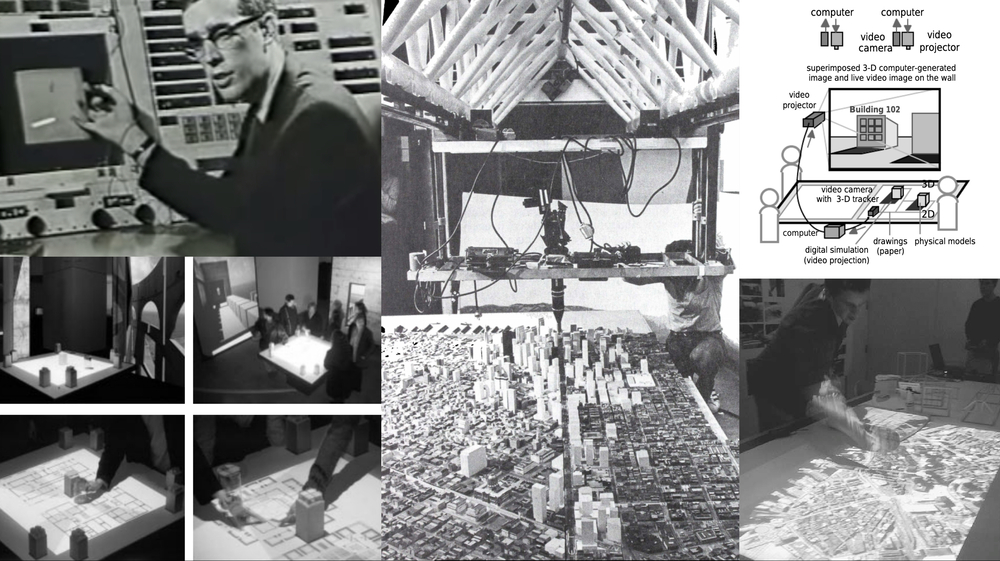
\includegraphics[width=0.9\textwidth]{figures/urbanHCI.jpg}
\end{center}
   \caption{Urban HCI milestones. Spanning over five decades, these systems aspired to combine the agility and rapidness of computational systems, with the ease of use and collaborative manner of tangible interfaces.    
   (top left) Sutherland, "Sketchpad" (1963),
   (bottom left)  Larson, "Louis I. Kahn: Unbuilt Masterworks" (1999),
   (center) Bosselmann, "The Berkeley Environmental Simulation Laboratory (1984),
   (right) Ben-Joseph, "luminous planning table" (2001)
   }
\label{fig:urbanHCI}
\end{figure}

{Since the 1960's, urban HCU researchers embraced the idea of collaborative and shared design environments, engaging professionals and non-professionals alike in the planning discourse \cite{Ben-Joseph2004, Ishii2008}. Although different in their design, purpose, and usage pattern, these tools share similar themes: (I) their design supports collaborative decision-making; (II) they promote playful and iterative design and feedback-loops; (III) and they are expected to respond in a near real-time manner \cite{Ullmer2010, Ben-Joseph2001, Snyder2003, mueller2018citizen}.}


\textbf{Multi-Stakeholders:}{A key component of urban HCI is the ability to engage multiple stakeholders at once \cite{Ben-Joseph2004}. Unlike traditional design and CAD interfaces, these platforms are built around large-scale, shared public spaces (physical or virtual) that can facilitate many participants. This can reduce the bureaucratic overhead of negotiating in different channels, and promote concise, result-driven participation sessions \cite{Ben-Joseph2001}. In the last few decades, urban HCI platforms were developed to facilitate collaborative urban design, augmented by computational analytics. Notably are the Environmental Simulation Laboratory (ESL) in Berkeley \cite{bosselmann1984berkeley}, URP \cite{underkoffler1999urp}, and the Augmented Urban Planning Workbench \cite{Ben-Joseph2004}, all built for collaboration in various stages of the urban process.}

{With the rise of internet, efforts to extend collaboration and participation beyond the limits of physical spaces brought these technologies to the virtual sphere. Using connected devices and shared virtual `sandboxes', planning discussions could also occur remotely, thus extending the number of potential participants in an order of magnitude \cite{Ben-Joseph2013, banerjee2011companion, green2019smart}. Advancements in Virtual, Augmented, and Mixed Reality, could allow remote participants to immersively understand, discuss, and reach consensus \cite{bulmer_how_2001}.}

\textbf{Iterative Urban Design:}{ }{Modern HCI technologies, including Virtual, Augmented, and Mixed Reality, Computer-Vision, advanced web applications, rapid-prototyping, and robotics can support iterative participation processes. Prior art include the I/O Bulb, The Clay Table and Sensetable \cite{Ishii2004, Ishii2002, Ishii2008} which converged the digital and the physical in seamless design-feedback loops. These systems allowed side-by-side comparison in both physical and virtual environments, in which each design iteration was only a starting point for an another design. Unlike linear design processes, this approach created a graph of potential design iterations with minimal overhead and virtually no cost. Different designs could then be evaluated for their trade-offs and Key Performance Indicators (KPIs), in an ``apples-to-apples'' comparison \cite{Ishii2002}. This kind of synchronous design process does not only expedite the designers work, but can also expose edge-cases and `out of the box' design solutions.}

\textbf{Interactive, Real-time Analytics:}
{Modern spatial analytics and urban-modeling techniques can serve urban HCI platforms with real-time data and high-end insights \cite{Kitchin2014, salganik_bit_2017}. Emerging modeling techniques, such as Machine-Learning and Deep-Learning, can expedite the investigation of complex planning scenarios and their effects on human dynamics, traffic, energy-use, or economic performance. Although some of these modelling techniques are not new, they were traditionally limited to experts, and their complexity required significant time and resources, making them less fit for real-time applications \cite{Foth2011}.}

\subsection {The Limits of a New Urban Process}

{Urban HCI platforms can transcend lengthy, inefficient, and costly planning processes. Current breakthroughs in Data Science could augment these systems with real-time urban analytics \cite{Barbosa-Filho2017}. Affordable computation and immersion technology can help better communicate design alternatives, their impacts and KPIs. Nevertheless, with the emergence of new technologies, new challenges arise, and several traditional issues still remain. This dissertation will address two aspects of urban HCI challenges: (I) technical limitations, such as accessibility, accuracy of models and data, and possible bias, as well as (II) the perils of `techno-utopia' and overreliance on technology. }


